\documentclass{beamer}
\mode<presentation> 
\usetheme{CambridgeUS}
\usecolortheme{seagull}
%\setbeamertemplate{headline}
%\setbeamertemplate{footline} 
% To remove the footer line in all slides uncomment this line

%\setbeamertemplate{footline}[page number] 
% To replace the footer line in all slides with a simple slide count uncomment this line

\setbeamertemplate{navigation symbols}{} 
% To remove the navigation symbols from the bottom of all slides uncomment this line

\usepackage{graphicx}
\usepackage{booktabs} 
\usepackage[round]{natbib}
\usepackage{verbatim}
\usepackage{subfigure}
\usepackage{multicol}

%----------------------------------------------------------------------
%	TITLE PAGE
%----------------------------------------------------------------------

\title[Narrative Conservatism]{Narrative Conservatism} % The short title appears at the bottom of every slide, the full title is only on the title page
\author[]{Juan Manuel Garc\'ia Lara, Beatriz Garc\'ia Osma, Fengzhi Zhu} % Your name
\institute[] % Your institution as it will appear on the bottom of every slide, may be shorth and to save space
{Universidad Carlos III de Madrid \\ % Your institution for the title page

	\medskip
	fzhu@emp.uc3m.es} % Your email address
\date{\today} % Date, can be changed to a custom date (\today)

\begin{document}
	
\begin{frame}
\titlepage % Print the title page as the first slide
\end{frame}

%-----------------------------------------------------------------
\begin{frame}
\frametitle{Outline}
\tableofcontents
\end{frame}

%-------------------------------------------------------------------
%	PRESENTATION SLIDES
%----------------------------------------------------
\section{Research Question and Contribution}
%------------------------------------------------

\begin{frame}
\frametitle{Research Question and Contribution}
\begin{itemize}
\item \textbf{Research Question}

\begin{itemize}
\item Whether narrative disclosure is conservative, i.e., whether narratives respond to bad news in a more complete, news-consistent and timely manner than good news?
\end{itemize}

\item \textbf{Contribution}

\begin{itemize}
	\item Filling the missing piece in conservatism literature by documenting the existence of narrative conservatism.
	\item Providing novel evidence to the debate regarding whether managers withhold bad news. 
	\item Relating to the broader literature on the informativeness of SEC filings.
	\item Adding to the literature on distinction and interaction between recognition and disclosure.
\end{itemize}
\end{itemize}
\end{frame}
%------------------------------------------------
\section{Theoretical Framework}
%------------------------------------------------
\begin{frame}
\frametitle{Theoretical Framework: Recognition and Disclosure}
\begin{itemize}
\item \textbf{Definition \citep{schipperRequiredDisclosuresFinancial2007}}
	
	\begin{itemize}
		\item Recognition: depictions in numbers with captions on the face of the financial statements
		\item Disclosure: display in the notes and supporting schedules that accompany financial statements
	\end{itemize}

\item \textbf{Reporting Requirement \citep{fasbStatementFinancialAccounting1984}}

	\begin{itemize}
		\item Recognition: an economic event can be recognized if it satisfies all of the following criteria
		\begin{itemize}
			\item Definition criterion
			\item Measurability criterion
			\item Relevance criterion
			\item Reliability criterion
		\end{itemize}
	% First, the item must meet the definition of an element of financial statements (definition criterion). Second, the item must have a relevant attribute measurable with sufficient reliability (measurability criterion). Third, the information about the item must be capable of making a difference in user decisions (relevance criterion). Fourth, the information must be representationally faithful, verifiable, and neutral (reliability criterion).
		\item Disclosure: can be deployed to disclose information that fails to meet certain recognition criteria
	\end{itemize}

\item \textbf{Role of Narratives} 

	\begin{itemize}
		\item Disclose information that cannot be recognized
		\item Explain recognized line items
	\end{itemize}

\end{itemize}
\end{frame}
%------------------------------------------------
\begin{frame}
\frametitle{Theoretical Framework: Conservatism}
\begin{itemize}
		
\item \textbf{Definition}

	\begin{itemize}
		\item Conditional and unconditional conservatism
		%``accountants' tendency to require a higher degree of verification to recognize good news as gains than to recognize bad news as losses" \citep*[p. 7]{basuConservatismPrincipleAsymmetric1997}
		%``accountants' preference for accounting methods that lead to lower reported values for shareholders' equity" \citep*[p. 8]{basuConservatismPrincipleAsymmetric1997}.
		\item Narrative conservatism: narratives responding to bad news in a more complete, news-consistent and timely manner than good news
	\end{itemize}

\item \textbf{Why do firms disclose or withhold bad news?}

\begin{itemize}
	\item Disclose: lower financing costs resulting from reduced information asymmetry, litigation risk due to the failure to disclose bad news in a timely manner and managers' personal incentive to manipulate firm performance downwards prior to stock option grant
	\item Withhold: managers' future career concern and performance-based compensation
\end{itemize}

\item \textbf{Hypotheses}

\begin{itemize}
	\item  \textbf{H1:} The total number of words in narrative disclosure is greater in response to bad news than good news.
	\item  \textbf{H2}: The marginal change of tone in narrative disclosure is greater in response to bad news than good news.
	\item  \textbf{H3}: The reporting time lag of narrative disclosure is shorter in response to bad news than good news.
\end{itemize}

\end{itemize}
\end{frame}
%------------------------------------------------
\begin{frame}
	\frametitle{Theoretical Framework: Conservatism Cont.}
	\begin{itemize}

\item \textbf{Is conservatism useful?}

	\begin{itemize}
		\item Valuation role: provide financial information about the reporting entity that is useful to existing and potential investors, lenders, and other creditors in making decisions about providing resources to the entity \citep[OB2]{fasbConceptualFrameworkFinancial2018b}
		\item Stewardship role: how efficiently and effectively the entity's management and governing board have discharged their responsibilities to use the entity's economic resources \cite[OB4]{fasbConceptualFrameworkFinancial2018b}
	\end{itemize}

\item \textbf{Is narrative conservatism useful?}
	\begin{itemize}
		\item We posit that narrative conservatism enhances contract efficiency and serves the stewardship role of accounting
		\item Testable hypotheses to be developed
	\end{itemize}

\end{itemize}
\end{frame}
%------------------------------------------------
\section{Research Design}
%------------------------------------------------
\begin{frame}
\frametitle{Research Design: Model}
\begin{itemize}

\item \textbf{Narrative Disclosure Corpora and News Proxy}

\begin{itemize}
	\item Narrative Disclosure Corpora are 10-Q and 8-K filings because they (a) are more credible, (b) have higher reporting threshold and (c) are more timely than other corporate communication channels.
	\item Heterogeneity between 10-Q and 8-K: (a) 10-Q is more diversified in content (b) 8-K is more timely.
	\item News proxy is stock returns, assuming market efficiency.
\end{itemize}

\item \textbf{Model Specification}
	\begin{itemize}
		\item Form 10-Q
		
		\begin{figure}[h]
			\centering
			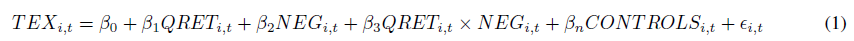
\includegraphics[width=0.75\linewidth]{eq1}
			\label{eq1}
		\end{figure}
	
		\item Form 8-K
		
		\begin{figure}[h]
			\centering
			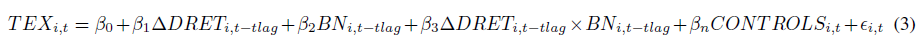
\includegraphics[width=0.8\linewidth]{eq3}
			\label{eq3}
		\end{figure}
	
		\begin{figure}[h]
			\centering
			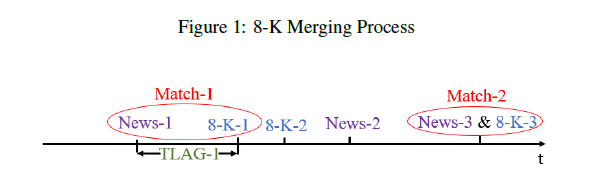
\includegraphics[width=0.6\linewidth]{fig1}
			\label{fig1}
		\end{figure}
	\end{itemize}

\end{itemize}
\end{frame}
%------------------------------------------------
\begin{frame}
\frametitle{Research Design: Data}

\begin{itemize}
	\item Historical financial and segment data from Compustat, stock returns from the Center for Research in Security Prices (CRSP) and analyst earnings forecasts data from I/B/E/S.
	
	\begin{figure}[h]
		\centering
		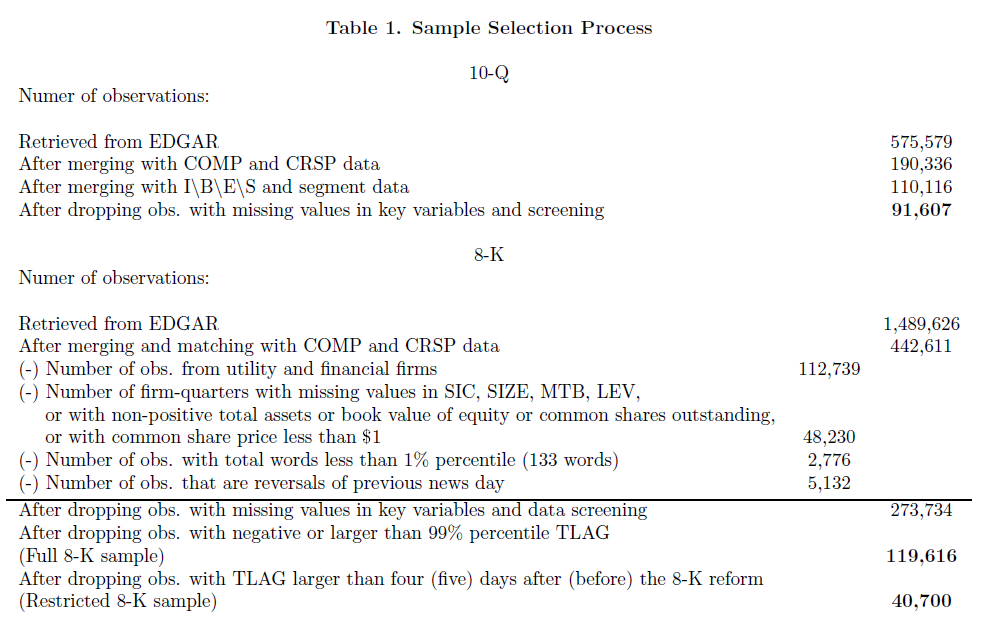
\includegraphics[width=0.8\linewidth]{tab1}
		\label{tab1}
	\end{figure}

\end{itemize}
\end{frame}
%------------------------------------------------
\section{Results}
%------------------------------------------------
\begin{frame}
\frametitle{Results: Summary Statistics}
\begin{figure}[h]
	\centering
	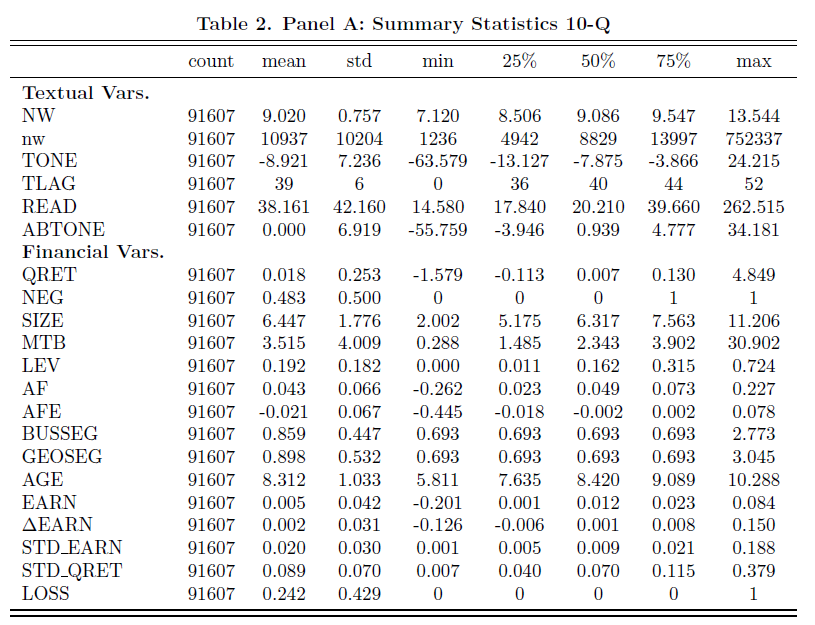
\includegraphics[width=0.7\linewidth]{tab2panA}
	\label{tab2panA}
\end{figure}

\end{frame}
%------------------------------------------------
\begin{frame}
	\frametitle{Results: Summary Statistics Cont.}
	\begin{figure}[h]
		\centering
		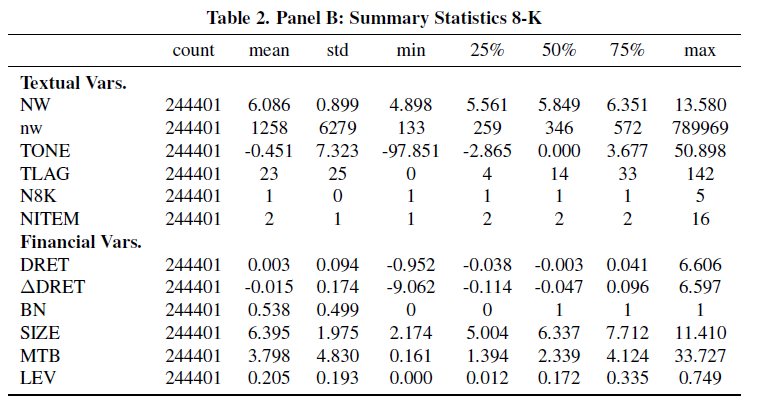
\includegraphics[width=0.65\linewidth]{tab2panB}
		\label{tab2panB}
	\end{figure}
	
\end{frame}
%------------------------------------------------
\begin{frame}
\frametitle{Results: 10-Q Main Results}
	\begin{figure}[h]
		\centering
		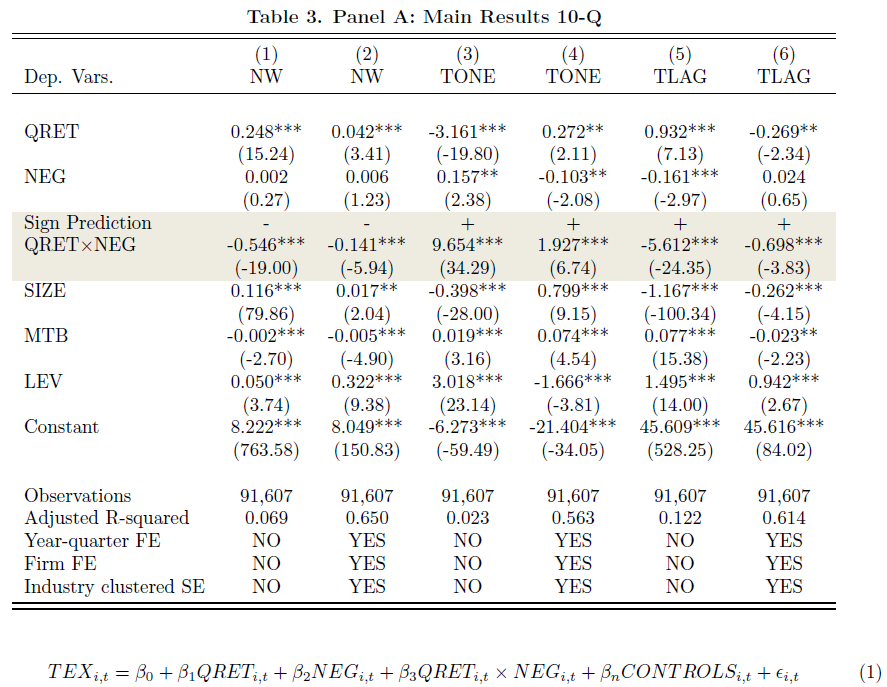
\includegraphics[width=0.7\linewidth]{tab3panA}
		\label{tab3panA}
	\end{figure}
\end{frame}
%------------------------------------------------
\begin{frame}
\frametitle{Results: 10-Q Additional Results}
\begin{multicols}{2}
	\begin{figure}[h]
	\centering
	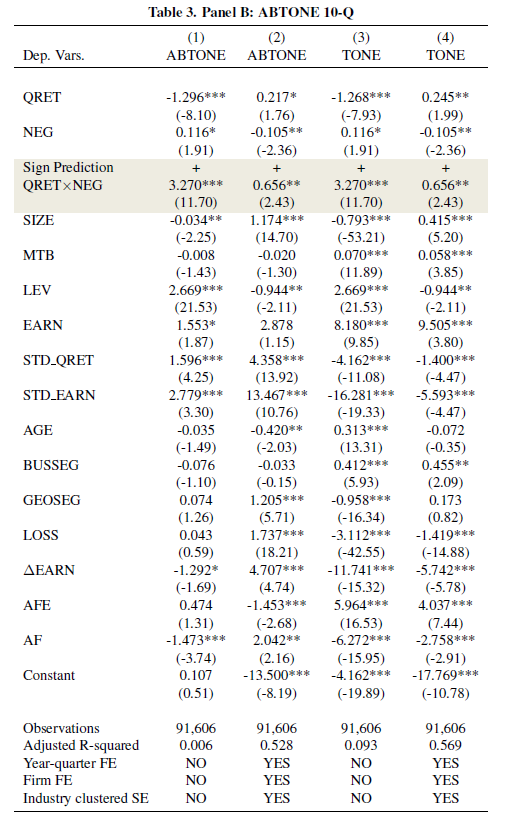
\includegraphics[width=0.79\linewidth]{tab3panB}
	\label{tab3panB}
	\end{figure}

	\begin{figure}[h]
	\centering
	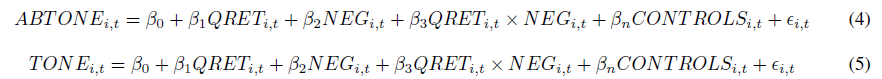
\includegraphics[width=1.05\linewidth]{tab3panBeq}
	\label{tab3panBeq}
	\end{figure}

	\begin{figure}[h]
	\centering
	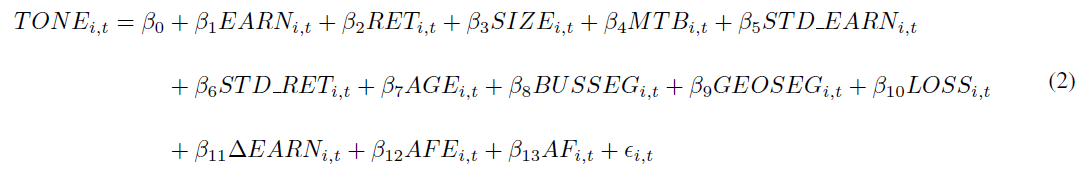
\includegraphics[width=1.05\linewidth]{eq2}
	\label{eq2}
	\end{figure}


\end{multicols}
\end{frame}
%------------------------------------------------
\begin{frame}
\frametitle{Results: 8-K Main Results}
	\begin{figure}[h]
	\centering
	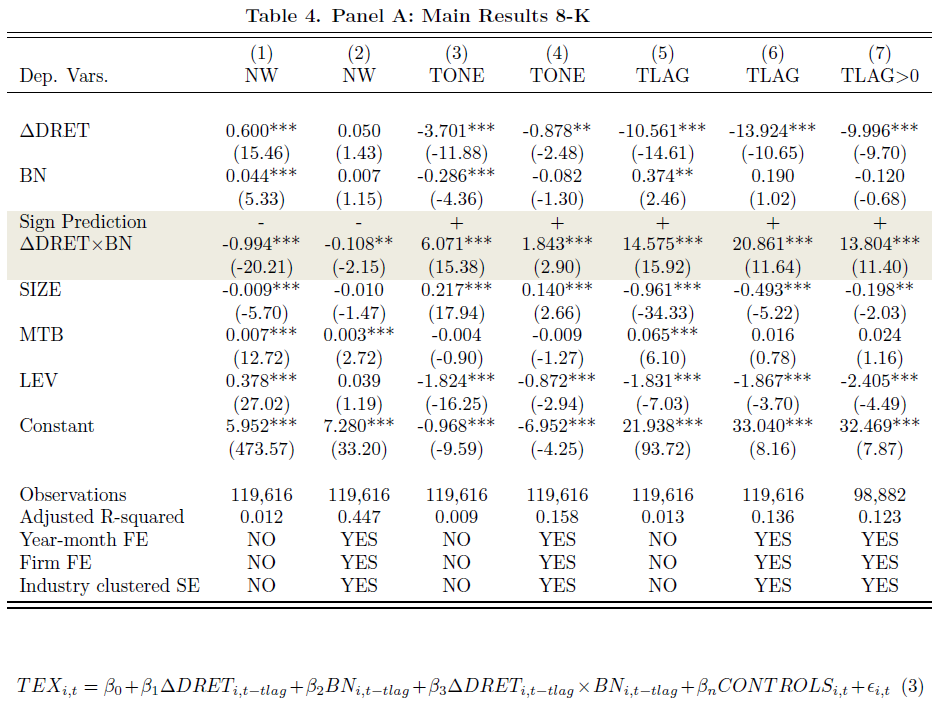
\includegraphics[width=0.75\linewidth]{tab4panA}
	\label{tab4panA}
	\end{figure}
\end{frame}
%------------------------------------------------
\begin{frame}
\frametitle{Results: 8-K Additional Results}
	\begin{figure}[h]
	\centering
	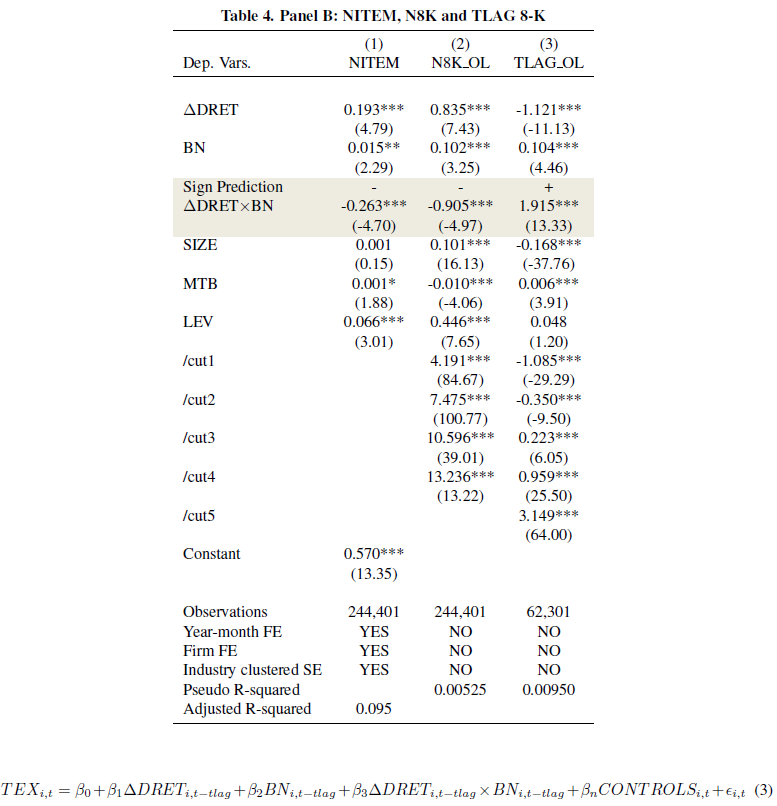
\includegraphics[width=0.6\linewidth]{tab4panB}
	\label{tab4panB}
	\end{figure}
\end{frame}
%------------------------------------------------
\section{Auxiliary Analysis}
%------------------------------------------------
\begin{frame}
\frametitle{Auxiliary Analysis}
\begin{itemize}
\item Managerial Incentives and Narrative Conservatism
	\begin{itemize}
		\item Litigation
		\item Compensation
		\item Option grant
		\item IPO
		\item Reg FD \citep{kothariManagersWithholdBad2009}
		\item Different Sections of Narratives in 10-Q
	\end{itemize}
\item Alternative News Proxy

\item Interaction Between Recognition and Narrative Conservatism

\item Economic Implications of Narrative Conservatism
\end{itemize}

\end{frame}
%------------------------------------------------
\section{Discussion}
%------------------------------------------------
\begin{frame}
\frametitle{Discussion}
\begin{itemize}
	\item \textbf{Conclusions}
	\begin{itemize}
		\item On average narratives have more number of words, greater marginal change of tone and shorter reporting time lag in response to bad news relative to good news, consistent with narratives being conservative.
		\item In addition, we show that firms emphasize bad news more than good news via 10-Q filings, and are more likely to report larger number of 8-K filings and 8-K items per day in response to bad news comparing to good news.
	\end{itemize}
	
	\item \textbf{Next Steps}
	\begin{itemize}
		\item Revise the writing part.
		\item Complete the (selected) auxiliary analyses.
	\end{itemize}
	
\end{itemize}

\end{frame}
%------------------------------------------------
\section{References}
%------------------------------------------------
\begin{frame}
\frametitle{Selected References}
\scriptsize
\bibliographystyle{plainnat}
\bibliography{NC_slides}
\end{frame}
%------------------------------------------------
\end{document}